\documentclass{lab}

\renewcommand{\AA}{\ensuremath{\mathring{A}}}

\begin{document}

\labtitle{5.5.1}{Измерение коэффициента ослабления потока $\gamma$-лучей в веществе и определение их энергии}{19~сентября~2019~г.}{26~сентября~2019~г.}

\section*{Постановка эксперимента}

\begin{quote}
	\textbf{{\normalsize Цель работы: }}
	с помощью сцинтилляционного счётчика измерить линейные коэффициенты ослабления потока
	$\gamma$-лучей  в свинце, железе и алюминии; по их величине определить энергию 
	$\gamma$-квантов.
\end{quote}

\begin{quote}
	\textbf{{\normalsize Оборудование: }}
	источник $ \gamma $-излучения, сцинтилляционный счетчик, секундомер.
\end{quote}

\section*{Теория}

	Гамма-лучи возникают при переходе возбуждённых ядер в более низкое энергетическое 
	состояние. Энергия $\gamma$-квантов обычно порядка~$10\div1000$ кэВ. Заряд и масса 
	$\gamma$-кванта равны нулю. Проходя через вещество, пучок $\gamma$-квантов ослабляется 
	по закону:
	\begin{equation}\label{eq:coef}
		I = I_0e^{-\mu l} ~~~ \Leftrightarrow ~~~
		I=I_0e^{-\mu' m_1},
	\end{equation}
	где $I, I_0$ - интенсивности прошедшего и падающего излучений, $l$~--~длина пути, 
	пройденного  пучком $\gamma$-лучей, $m_1$~--~масса пройденного вещества на единицу 
	площади, $\mu$~и~$\mu'$~--~константы, зависящие от среды ($[\mu] = \text{см}^{-1}$, 
	$[\mu'] = \text{см}^{2}/\text{г}$). $\mu'$, в отличие от~$\mu$, не зависит от плотности 
	среды. Ослабление потока $\gamma$-лучей в веществе связано с тремя эффектами: 
	фотоэлектрическим поглощением, комптоновским рассеянием и генерацией 
	электрон-позитронных пар.\\
	
	\textbf{Фотоэлектричекое поглощение}
	
	При столкновении $\gamma$-квантов с электронами внутренних атомных оболочек может 
	происходить поглощение квантов. Свободные (наружные) электроны не могут поглощать 
	кванты. Вероятность $dP_\text{ф}$ фотоэлектрического поглощения $\gamma$-квантов: 
	\[ dP_\text{ф}=\sigma_\text{ф} n_1 dl, \]
	где $dl$~---~длина пути, $n_1$~---~плотность внутренних  электронов, 
	$\sigma_\text{ф}$~---~поперечное сечение фотоэлектрического поглощения.
	\[ \mu_\text{ф}=\sigma_\text{ф}n_1, \]	
	$\mu_\text{ф}$~---~коэффициент поглощения для фотоэффекта $\mu$ из уравнения \eqref{eq:coef}.
	
	Фотоэффект является доминирующим механизмом поглощения $\gamma$-квантов при не очень 
	высоких энергиях. Его вероятность зависит от энергии лучей и заряда  ядер.
	\begin{figure}[H]
		\centering
		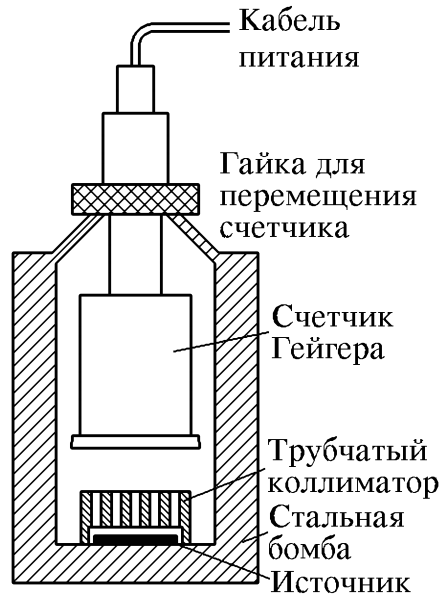
\includegraphics[width=0.45\linewidth]{1}
		\caption{Зависимость сечения фотоэффекта от энергии $\gamma$-квантов.}
	\end{figure}

	\textbf{Комптоновское рассеяние}
	
	Комптоновское рассеяние~--~упругое столкновение $\gamma$-кванта с электроном. Оно может 
	происходить на свободных/слабосвязанных электронах. Эффект Комптона становится 
	существенным, когда энергия квантов становится много больше энергии связи электронов в 
	атоме. В этом случае сечение комптон-эффекта:
	\begin{equation}
	 \sigma_K=\pi r^2 \dfrac{mc^2}{\hbar \omega}\left(\ln\frac{2\hbar\omega}{mc^2}+\frac{1}{2}\right),
	\end{equation}
	где $r\simeq 2.8 \cdot 10^{-13}$ см~--~классический радиус электрона, $m$~--~его масса.
	
	Эффект Комптона приводит не к поглощению, а к рассеянию $\gamma$-квантов и уменьшению их энергии.\\
	
	\textbf{Образование пар}
	
	При энергиях $\gamma$-лучей больше 1.02 МэВ становится возможным поглощение лучей, 
	связанное с образованием электрон-позитронных пар. Оно возникает в электрическом поле 
	ядер. Вероятность этого процесса приблизительно пропорциональна $Z^2$.\\
	
	\textbf{Полный коэффициент ослабления потока $\gamma$-лучей}
	
	Полный коэффициент ослабления потока лучей равен сумме коэффициентов для трёх 
	рассмотренных процессов. 
	
	\begin{figure}[H]
		\centering
		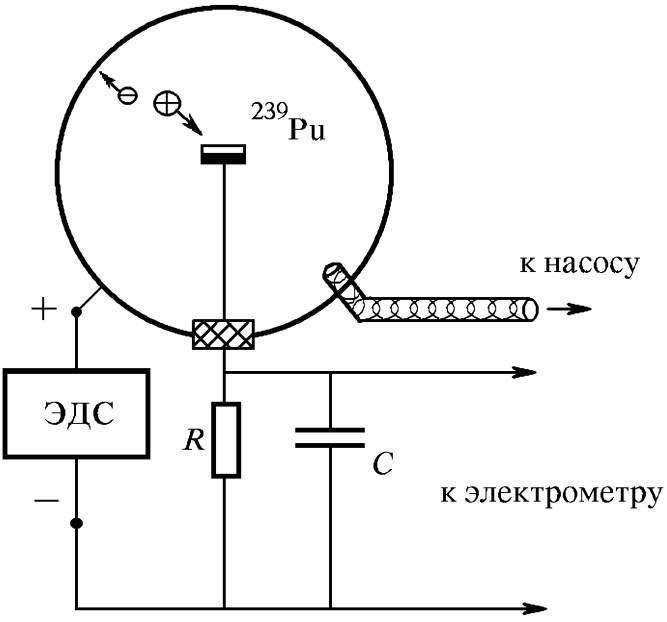
\includegraphics[width=0.5\linewidth]{2}
		\caption{Полные коэффициенты ослабления потока $\gamma$-лучей в алюминии, железе и свинце.}
	\end{figure}
	
	Полный коэффициент ослабления:
	
	\begin{equation}
	\mu=\frac{1}{l}\ln\frac{N_0}{N}
	\end{equation}
	
	В работе определяются толщина образца $l$, число падающих частиц $N_0$ и число прошедших частиц $N$.
	
\newpage
	
\section*{Экспериментальная установка}

	Схема установки, используемой в работе, показана на рисунке \ref{scheme1}. Свинцовый 
	коллиматор выделяет узкий почти параллельный пучок $ \gamma $-квантов, проходящий через 
	набор поглотителей. Сигналы от счетчика усиливаются и регистрируются пересчетным 
	прибором. Высоковольтный выпрямитель обеспечивает питание сцинтилляционного счетчика.
	
	\begin{figure} [h!]
		\centering
		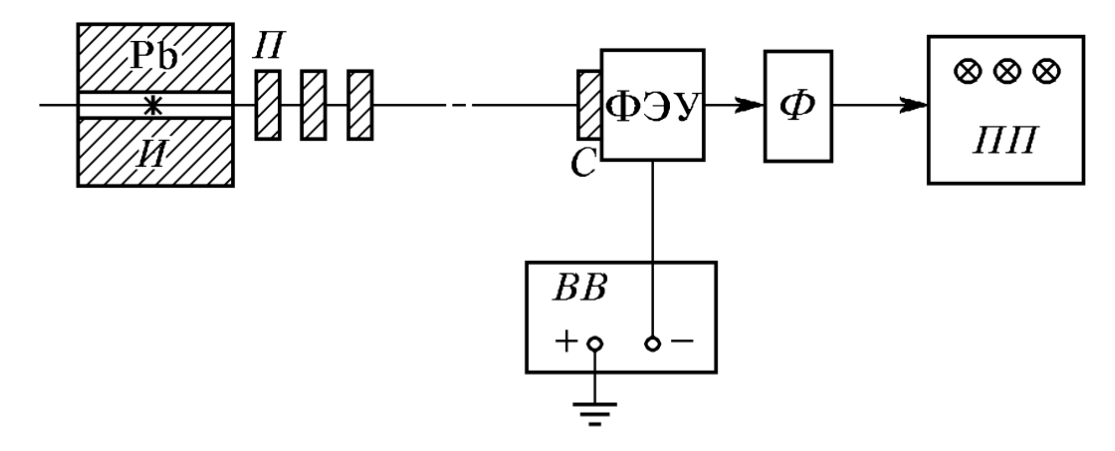
\includegraphics[width=0.8\linewidth]{3}
		\caption{Блок-схема установки, используемой для измерения коэффициентов ослабления 
			потока $\gamma$-лучей; Pb~---~свинцовый контейнер с коллиматорным каналом; 
			П~---~набор поглотителей, ПП~---~пересчётный прибор; С~---~сцинтиллятор 
			(кристалл NaI(Tl)); ВВ~---~высоковольтный выпрямитель, 
			Ф~---~формирователь-выпрямитель; И~---~источник $\gamma$-лучей}
		\label{scheme1}
	\end{figure}
	
	\begin{figure} [h!]
		\centering
		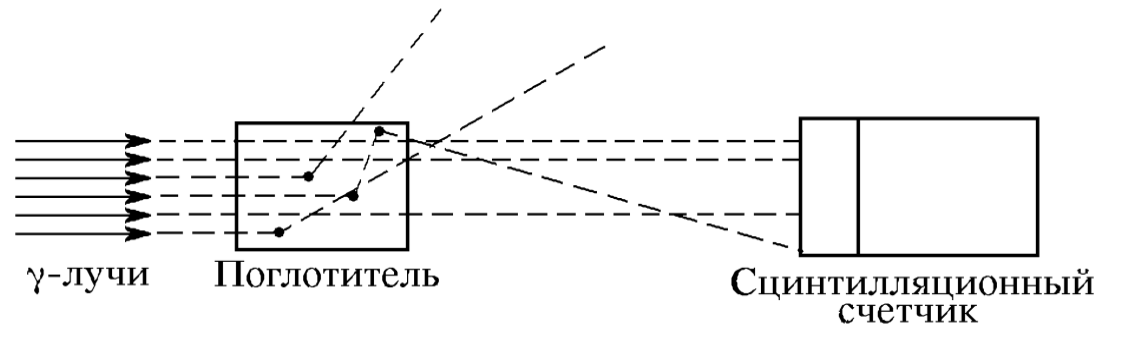
\includegraphics[width=0.9\linewidth]{4}
		\caption{Схема рассеяния $\gamma$-квантов в поглотителе}
	\end{figure}

\newpage

\section*{Выполнение работы}

\begin{enumerate}
\item
Посмотрим на излучение при открытом и закрытом источниках в течение 5~с. Точность измерений 
счетчиком везде примем равной $ 0.3\% $.
\begin{table}[H]
	\centering
	\begin{tabular}{|c|ccc|}
		\hline
		$ N(открыт) $ & 39000 & 38000 & 38000 \\
		$ N(закрыт) $ & 95    & 85    & 95    \\ \hline
	\end{tabular}
	\caption{Время измерения $ t=5~с $.}
	\label{tab0}
\end{table}

	
\item 
Получим зависимость поглащения $ \gamma $-лучей в алюминии, железе и свинце. Измерения 
проведем за время $ t = 20~с $. Для каждого случая $ l $ -- длина препятствия.

\begin{table}[H]
	\centering
	\begin{tabular}{|c|cccccccc|}
		\hline
		$ l,~см $ & 0.0    & 2.0   & 4.0   & 6.0   & 8.0   & 10.0  & 12.0  & 14.0 \\
		$ N,~шт $ & 149727 & 97197 & 65068 & 43321 & 28403 & 18834 & 12633 & 8774 \\ \hline
	\end{tabular}
	\caption{Алюминий. Погрешность измерения $ l: \varepsilon = 0.8\% $.}
	\label{tab1}
\end{table}

\begin{table}[H]
	\centering
	\begin{tabular}{|c|cccccc|}
		\hline
		$ l,~см $ & 0.0    & 1.0   & 2.0   & 3.0   & 4.0   & 5.0  \\
		$ N,~шт $ & 148843 & 87834 & 47679 & 26980 & 15891 & 8877 \\ \hline
		$ l,~см $ & 6.0  & 7.0  & 8.0  & 9.0  & 10.0 & 11.0 \\
		$ N,~шт $ & 5438 & 3238 & 2008 & 1384 & 987  & 710  \\ \hline
	\end{tabular}
	\caption{Железо. Погрешность измерения $ l: \varepsilon = 0.9\% $.}
	\label{tab2}
\end{table}

\begin{table}[H]
	\centering
	\begin{tabular}{|c|cccccc|}
		\hline
		$ l,~см $ & 0.0    & 0.5   & 1.0   & 1.5   & 2.0   & 2.5  \\
		$ N,~шт $ & 152572 & 84759 & 50209 & 28060 & 16262 & 9812 \\ \hline
		$ l,~см $ & 3.0  & 3.5  & 4.0  & 4.5  & 5.0  & 5.5 \\
		$ N,~шт $ & 6023 & 3687 & 2370 & 1613 & 1175 & 977 \\ \hline
	\end{tabular}
	\caption{Свинец. Погрешность измерения $ l: \varepsilon = 1.3\% $.}
	\label{tab3}
\end{table}

\item
Посмотрим на излучение рядом с источником в течение 10~с, а также на показания счетчика при 
закрытом источнике в зависимости от времени.
\begin{table}[H]
	\centering
	\begin{tabular}{|c|ccc|}
		\hline
		$ N(рядом) $  & 1027491 & 986199 & 973175 \\ \hline
		$ t,~с $      & 100     & 200    & 300    \\
		$ N(закрыт) $ & 1780    & 3663   & 5464   \\ \hline
	\end{tabular}
	\caption{Измерение фона.}
	\label{tab00}
\end{table}

\item
Построим графики зависимостей логарифма числа прошедших частиц от толщины образца для 
каждого материала. Также не забудем учесть фоновые излучения, отнимем из числа срабатывания 
счетчика $ N_{фон} = 364 $.

\begin{figure}[H]
	\centering
	\begin{tikzpicture}
	
	\pgfplotstableread{
		 X	    Y		x-err	y-err
		 0	11.91		0.1		0.05
		 2	11.48		0.1		0.05
		 4	11.08		0.1		0.05
		 6	10.67		0.1		0.05
		 8	10.24		0.1		0.05
		 10	 9.82		0.1		0.05
		 12	 9.41		0.1		0.05
		 14	 9.04		0.1		0.05
	}{\mytable}
	
	\begin{axis}[
	width = 0.8\textwidth,
	grid = major,
	xlabel = $ l\text{, см} $,
	ylabel = $ \ln (N) $,
	ymin = 9,
	ymax = 12,
	xmin = 0,
	xmax = 14
	]
	
	\addplot[
	only marks,
	color = red,
	mark = *,
	error bars/.cd,
	x dir = both,
	x explicit,
	y dir = both,
	y explicit
	]
	table[
	x error = x-err,
	y error = y-err
	] {\mytable};
	
	\addplot[
	mark = none,
	color = red
	]
	table[
	y = {create col/linear regression={y=Y}}
	] % compute a linear regression from the
	{\mytable};
	
	\end{axis}
	\end{tikzpicture}
	\caption{Алюминий.}
	\label{g_1}
\end{figure}

\begin{figure}[H]
	\centering
	\begin{tikzpicture}
	
	\pgfplotstableread{
		X	    Y		x-err	y-err
		0	11.91		0.1		0.1
		1	11.38		0.1		0.1 
		2	10.76		0.1		0.1
		3	10.19		0.1		0.1
		4	 9.65		0.1		0.1
		5	 9.05		0.1		0.1
		6	 8.53		0.1		0.1
		7	 7.96		0.1		0.1
		8	 7.40		0.1		0.1
		9	 6.93		0.1		0.1
		10	 6.43		0.1		0.1
		11	 5.85		0.1		0.1
	}{\mytable}
	
	\begin{axis}[
	width = 0.8\textwidth,
	grid = major,
	xlabel = $ l\text{, см} $,
	ylabel = $ \ln (N) $,
	ymin = 5,
	ymax = 12,
	xmin = 0,
	xmax = 11
	]
	
	\addplot[
	only marks,
	color = red,
	mark = *,
	error bars/.cd,
	x dir = both,
	x explicit,
	y dir = both,
	y explicit
	]
	table[
	x error = x-err,
	y error = y-err
	] {\mytable};
	
	\addplot[
	mark = none,
	color = red
	]
	table[
	y = {create col/linear regression={y=Y}}
	] % compute a linear regression from the
	{\mytable};
	
	\end{axis}
	\end{tikzpicture}
	\caption{Железо.}
	\label{g_2}
\end{figure}

\begin{figure}[H]
	\centering
	\begin{tikzpicture}
	
	\pgfplotstableread{
		X	    Y		x-err	y-err
		0.0	11.93		0.07		0.15
		0.5	11.34		0.07		0.15
		1.0	10.82		0.07		0.15
		1.5	10.23		0.07		0.15
		2.0	 9.67		0.07		0.15
		2.5	 9.15		0.07		0.15
		3.0	 8.64		0.07		0.15
		3.5	 8.11		0.07		0.15
		4.0	 7.60		0.07		0.15
		4.5	 7.13		0.07		0.15
		5.0	 6.70		0.07		0.15
		5.5	 6.42		0.07		0.15
	}{\mytable}
	
	\begin{axis}[
	width = 0.8\textwidth,
	grid = major,
	xlabel = $ l\text{, см} $,
	ylabel = $ \ln (N) $,
	ymin = 6,
	ymax = 12,
	xmin = 0,
	xmax = 5.5
	]
	
	\addplot[
	only marks,
	color = red,
	mark = *,
	error bars/.cd,
	x dir = both,
	x explicit,
	y dir = both,
	y explicit
	]
	table[
	x error = x-err,
	y error = y-err
	] {\mytable};
	
	\addplot[
	mark = none,
	color = red
	]
	table[
	y = {create col/linear regression={y=Y}}
	] % compute a linear regression from the
	{\mytable};
	
	\end{axis}
	\end{tikzpicture}
	\caption{Свинец.}
	\label{g_3}
\end{figure}

\item 

Из графиков находим:
\begin{equation}
\mu_\text{Al} = (0.206~\pm~0.001)~см^{-1} ~~~
\mu_\text{Fe} = (0.551~\pm~0.003)~см^{-1} ~~~
\mu_\text{Pb} = (1.025~\pm~0.007)~см^{-1}
\end{equation}

\item 
Используя найденные коэффициенты ослабления и табличные данные, определили среднюю энергию $ 
\gamma $-лучей, испускаемых источником:
\begin{equation}
E_{\gamma} \sim 0.5 \div 0.6~МэВ
\end{equation}

\end{enumerate}

\subsection*{Итоги}

Исследовали поглощение $\gamma$-лучей в алюминии, железе и свинце. Получили линейные 
зависимости логарифма прошедших частиц от толщины образцов и по ним определили линейные 
коэффициенты ослабления $\mu$, а также среднюю энергию $\gamma$-лучей, испускаемых 
источником.

\end{document}